\documentclass{sig-alternate}
\usepackage{epsfig}
\usepackage{epsfig}
\usepackage{amsmath}
\usepackage{algorithm}
\usepackage{algorithmic}

\title{Affine Dependence Analysis \\ for Cyclo-Static Dataflow Graphs}
\numberofauthors{1}
\author{
\alignauthor \vspace{-18pt}
William Thies,
Jasper Lin,
and Saman Amarasinghe \\
	\vspace{8pt}
	\{thies, jasperln, saman\}@lcs.mit.edu \\
	\vspace{8pt}
	Laboratory for Computer Science \\
	Massachusetts Institute of Technology}

\begin{document}

\newtheorem{definition}{Definition}

\maketitle

  %%%%%%%%%%%%%%%%%%%%%%%%%%%%%%%%%%%%%%%%%%%%%%%%%%%%%%%%%%%

  \newcommand{\mt}[1]{\mbox{\it #1}}
  \newcommand{\todo}[1]{\framebox{\bf #1}}
  \newcommand{\dep}[0]{Dependence Frontier}                % The full name for the dependence function.
  \newcommand{\DP}[0]{\textsc{Frontier}}                   % Abbrevation for dependence function.
  \newcommand{\DEP}[2]{\DP_{#1 \small{\rightarrow} #2}}    % Math notation for dependence function.
  \newcommand{\sssection}[1]{\medskip \noindent {\bf #1} \smallskip}

  \begin{abstract}
    As DSP programming is becoming more complex, there is an increasing
need for high-level abstractions that can be efficiently compiled.
Toward this end, we present a set of aggressive optimizations that
target linear sections of a stream program.  Our input language is
StreamIt, which represents programs as a hierarchical graph of
autonomous filters.  A filter is linear if each of its outputs can be
represented as an affine combination of its inputs.  Linear filters
are common in DSP applications; examples include FIR filters,
expanders, compressors, FFTs and DCTs.

We present a linear extraction analysis that automatically detects
linear filters based on the C-like code in their {\tt work} function.
Once linear filters are identified, we show how neighboring nodes can
be collapsed into a single linear representation, thereby eliminating
many redundant computations.  Also, we describe a method for
automatically translating linear nodes into the frequency domain,
thereby yielding algorithmic savings for convolutional filters.

We have completed a fully-automatic implementation of the above
techniques as part of the StreamIt compiler, and we demonstrate
performance improvements that average 400\% over our benchmark
applications.




  \end{abstract}

  \section{Introduction}

Applications that are structured around some notion of a ``stream''
are becoming increasingly important and widespread.  There is evidence
that streaming media applications are already consuming most of the
cycles on consumer machines \cite{Rix98}, and their use is continuing
to grow.  In the embedded domain, applications for hand-held
computers, cell phones, and DSP's are centered around a stream of
voice or video data.  The stream abstraction is also fundamental to
high-performance applications such as intelligent software routers,
cell phone base stations, and HDTV editing consoles.

Despite the prevalence of these applications, there is surprisingly
little language and compiler support for practical, large-scale stream
programming.  Of course, the notion of a stream as a programming
abstraction has been around for decades \cite{SICP}, and a number of
special-purpose stream languages have been designed (see
\cite{survey97} for a review).  Many of these languages and
representations are elegant and theoretically sound, but they often
lack features and are too inflexible to support straightforward
development of modern stream applications, or their implementations
are too inefficient to use in practice.  Consequently, most
programmers turn to general-purpose languages such as C or C++ to
implement stream programs.

There are two reasons that general-purpose languages are inadequate for
stream programming.  Firstly, they are a mismatch for the application
domain.  That is, they do not provide a natural or intuitive
representation of streams, thereby having a negative effect on
readability, robustness, and programmer productivity.  Moreover, because
the widespread parallelism and regular communication patterns of data
streams are left implicit in general-purpose languages, compilers are
not stream-conscious and do not perform stream-specific optimizations.
As a result, performance-critical loops are often hand-coded in a
low-level assembly language and must be re-implemented for each target
architecture.  This practice is labor-intensive, error-prone, and very
costly.

Secondly, general-purpose languages are a mismatch for the emerging
class of grid-based architectures \cite{smartmemories,rawshort,trips} that
are especially well-suited for stream processing.  Perhaps the primary
appeal of C is that it provides a ``common machine language'' for
von-Neumann architectures.  That is, it abstracts away the
idiosyncratic differences between machines, but encapsulates their
common properties: a single program counter, arithmetic operations,
and a monolithic memory.  However, for grid-based architectures, the
von-Neumann model no longer holds, as there are multiple instruction
streams and distributed memory banks.  Thus, C no longer serves as a
common machine language--in fact, it provides the wrong abstraction
for the underlying hardware, and architecture-specific directives are
often needed to obtain reasonable performance.  Again, this greatly
complicates the job of the programmer and hampers portability.

StreamIt is a language and compiler specifically designed for modern
stream programming.  The StreamIt language has two goals: first, to
provide high-level stream abstractions that improve programmer
productivity and program robustness within the streaming domain, and
second, to serve as a common machine language for grid-based
processors.  At the same time, the StreamIt compiler aims to perform
stream-specific optimizations to achieve the performance of an expert
programmer.

This paper motivates, describes, and justifies the high-level language
features of StreamIt, version 1.0.  The major limitation of StreamIt
1.0 is that all flow rates in the streams must be static; applications
such as compression that have dynamically varying flow rates will be
the subject of future work.  A large set of applications can be
implemented with static rates, and while dynamic rates will require a
different runtime model, it will still be essential to fully analyse
and optimize static sub-sections in order to obtain high performance.

The paper is organized as follows. In Section {\ref{sec:domain}}, we
characterize the domain of streaming programs that motivates the
design of StreamIt, and in Section~\ref{sec:overview} we describe the
language features in detail.  We present an in-depth example of a
software radio in Section~\ref{sec:example}, preliminary results in
Section~\ref{sec:results}, related work in Section~\ref{sec:related},
and conclusions in Section~\ref{sec:conc}.


  \section{Related Work}
\label{sec:related}

Software pipelining for clustered vliws \cite{qian02}.

The Imagine stream processor~\cite{rixner98bandwidthefficient}
supports a time-multiplexed execution model.  The architecture
contains 48 parallel ALU's organized into 6 VLIW clusters.  The
programming model requires the programmer to write computation filters
in Kernel-C and stitch them together using Stream-C.  Because the
execution unit is data-parallel, the compiler uses time multiplexing
to execute a single filter at a time across all of the parallel
clusters.  While this provides perfect load balancing and high
arithmetic utilization when there is abundant data parallelism, it
suffers when a filter has retained state or data-dependences between
iterations.  Moreover, architectures based solely on
time-multiplexing do not scale spatially, as there are global wires
orchestrating the parallel execution units. 

Previous work in compiling StreamIt to Raw has taken a purely space
multiplexed approach~\cite{streamit-asplos}.  In this model, a single
filter was mapped to each execution tile.  To support applications
with more filters than execution tiles, a partitioning algorithm was
employed to adjust the granularity of the graph by fusing adjacent
filters into one.

Previous work in scheduling computation graphs to parallel targets
have focused on dynamic techniques \cite{SDFSched, SDFSched2,
may87communicating, DAGSched}. In general, multiple graph nodes are
{\it clustered} onto a single computational node and scheduled
dynamically.  

Our work, unlike most previous work in this field,
models link contention and topography.  Furthermore, StreamIt graphs
are implicitly formed of loops so we can apply loop scheduling
techniques such as software pipelining to build our schedules.

%The problem of instruction scheduling for MIMD and VLIW architectures
%is similar to the problem tackled by the space-time compiler.  ILP
%compilers for clustered VLIW architectures~\cite{Bulldog, Multiflow}
%are decomposed into stages that are analogous to the stages of the
%SpaceTime compiler.  These compilers must partition or cluster
%instructions, assign instructions to processors, and then schedule the
%instructions.  

Previous work on software pipelining has focused on scheduling machine
instructions in a loop \cite{lam-softpipe, rau-softpipe} to a
uniprocessor target.  The algorithms devised must account for tight
resource constraints and complex instruction dependences.  Our
software-pipelining problem is much less constrained, a traditional
modulo scheduling algorithm can not effectively take advantage of this
flexibility.  Previous work on ILP scheduling for the Raw
architectures ~\cite{lee98spacetime} also bears similarity.  However,
these compilers schedule graphs of fine-grained instructions. The
partitioning and scheduling heuristics are mindful of a different set
of constraints including different types of dynamism and less regular
communication patterns as compared to StreamIt graphs.

As far as we know, we are the first to apply loop-level scheduling
techniques to the problem of scheduling coarse-grained task graphs.

% \cite{cheops-thesis}
%   http://web.media.mit.edu/~kung/publication/thesis.pdf
%
% other possible things to cite:
%  http://portal.acm.org/citation.cfm?id=801721&dl=ACM&coll=portal
%  http://www.csrl.unt.edu/~kavi/Research/ica3pp156.pdf
%  http://cdmetcalf.home.comcast.net/papers/cop/node1.html#SECTION00010000000000000000

  \section{Notation}
\label{sec:pcg}

%% \begin{table}[t]
%% \small
%% \begin{center}
%% \begin{tabular}{|c|c|c|c|c|c|} \hline
%% Model of Computation & Items on Channels & Nodes with & Nodes with & Cyclic Steady \\
%%                      & at Start & Push $\ne$ Pop & Peek $>$ Pop & State Phases \\
%% \hline \hline
%% Synchronous Dataflow~\cite{LM87-i} & X & X & & \\
%% \hline
%% Cyclo-Static Dataflow~\cite{BELP96} & X & X & & X \\
%% \hline
%% Computation Graphs~\cite{KM66} & X & X & X & \\
%% \hline
%% Phased Computation Graphs & X & X & X & X \\
%% \hline
%% \end{tabular}
%% \vspace{-6pt}
%% \caption{\protect\small Models of Computation for Dataflow Graphs.}
%% \label{tab:models}
%% \vspace{-12pt}
%% \end{center}
%% \end{table}

In this section we give our notation for representing programs in the
framework of Cyclo-Static Dataflow.

\subsection{Cyclo-Static Dataflow Graph}
Formally, a Cyclo-Static Dataflow Graph is a directed graph with the
following components:
\begin{itemize}

\item Nodes $n_1 \dots n_{m_n}$.

\item Channels $c_1 \dots c_{m_c}$, where each channel is directed
from a given node $n_a$ to a given node $n_b$.

\item The number of phases $\mt{num}(n)$ that node $n$ exhibits.  For
all $n$, $\mt{num}(n) \ge 1$.

\item Non-negative integers $U(c, p)$ and $O(c, p)$, which give the
number of items pushed and popped, respectively, over channel $c$
during the $p$'th phase.

%% % NOTE that this is overly cautious within loops... could have smaller A(c)
%% \item A non-negative integer $A(c)$ indicating the number of items
%%   that are initially present on channel $c$.  There must be enough
%%   items present on $c$ to ensure a node can execute all of its phases
%%   during a steady-state schedule.  This constraint can be posed
%%   conservatively\footnote{A more precise formulation is as follows.
%%   For a given channel $c$, set $Emax_0 = 0$ and $Emax_{p+1} =
%%   max(maxE_p, E(c,p) + \sum_{i=0}^{p} O(c,p))$ for all $p \in [0,
%%   num(c) - 1]$.  Then $A(c) \ge Emax_{num(c)-1} -
%%   \sum_{i=0}^{num(c)-1} O(c,p)$.} as $A(t) \ge max_p (E(c,p) -
%%   o(c,p))$.

\end{itemize}

\subsubsection{Execution Model}

We give an informal description of the execution semantics of a
CSDG.An execution consists of a sequence of atomic {\it firings} of
nodes in the graph.  The effect of firing a given node depends on its
phase, which is a local state of the node.  At the start of execution,
each node is in phase 0, and each channel $c$ contains 0 items.

Let us consider a node $n$ that is in phase $p$.  It is legal for $n$
to fire if $p \in [0, \mt{num}(n)-1]$ and, for each channel $c_{in}$
directed into $n$, there are at least $O(c_{in}, p)$ items on
$c_{in}$.  The effect of this firing is to consume $O(c_{in}, p)$
items from each channel $c_{in}$ directed into $n$; to produce
$U(c_{out}, p)$ new items on each channel $c_{out}$ directed out of
$n$; and to advance the phase $p$ of $n$ to $(p +
1)~\mt{mod}~\mt{num}(n)$.

From the starting state of the graph, execution proceeds via an
infinite sequence of node firings.  The order of node firings is
constrained only by the conditions given above.

\subsection{Cyclo-Static Dataflow Program}

The CSDG described above is a representation for a graph, treating
each node and channel as a black box.  Here we introduce some notation
for the internals of the nodes, as well as the ordering of items on
the channels.  We refer to the aggregate model as a Cyclo-Static
Dataflow Program (CSDP).  Before describing a CSDP, we will need some
additional notation:
\begin{itemize}

\item We assume that all items passed over channels are drawn from the
same domain of values ${\cal V}$.

\item An array type\footnote{To simplify the presentation, we allow
ourselves a slight abuse of notation by sometimes using arrays instead
of enumerating individual elements.  Our definitions could be expanded
into strict element-wise SARE's without any fundamental change to the
technique.} of length $n$ and element type $\tau$ is denoted by
$\tau[n]$.  Given a two-dimensional array $A$ of type $\tau[n][m]$,
$A[i][*]$ denotes the $m$-element array comprising the $i$'th row of
$A$.

\item $\mt{num\_in}(n)$ (resp. $\mt{num\_out}(n)$) denotes the number of
channels that are directed into (resp. out of) node $n$.

\item $\mt{chan\_in}(n)$ (resp. $\mt{chan\_out}(n)$) denotes the list of
channels that are directed into (resp. out of) node $n$.

\item $\mt{pos\_in}(n, c)$ (resp. $\mt{pos\_out}(n, c)$) denotes the
position of channel $c$ in $\mt{chan\_in}(n)$
(resp. $\mt{chan\_out}(n)$.  That is, $\mt{chan\_out}(n)[\mt{pos\_out(n,
c)}] = c$.

\end{itemize}

\noindent A Cyclo-Static Dataflow Program (CSDP) consists of the
following:
\begin{itemize}

\item A Cyclo-Static Dataflow Graph $G = (\{n_1$ $\dots$ $n_{m_n}\},$
$\{c_1$ $\dots$ $c_{m_c}\},$ $\mt{num},$ $U,$ $O)$ describing the
nodes, channels, and I/O rates of the program (see
Section~\ref{sec:pcg}).  Each channel $c = (n_a, n_b)$ is a FIFO
queue; $n_a$ pushes items onto the back of $c$ and $n_b$ consumes
items from the front of $c$.

%% \item The initial values $I(c)$ that are enqueued onto channel $c$ at
%% the start of execution.  Since there are $A(c)$ initial values on
%% channel $c$, $I(c)$ has type ${\cal V}[A(c)]$.
%An initialization function $I(c)$ that returns an array of
%length $A(c)$, the elements of which are enqueued onto channel $c$ at
%the start of execution.  The procedure $I(c)$ takes no arguments; its
%signature is $\mt{void} {\small \rightarrow} {\cal V}[A(c)]$.
%
\item A work function $W(n, p)$ that represents the computation of
node $n$ in phase $p$.  The signature of $W(n, p)$ is:
{\scriptsize
\begin{equation*}
[{\cal V}[O(\mt{chan\_in}(n)[1], p)], \dots, {\cal V}[O(\mt{chan\_in}(n)[\mt{num\_in}(n)], p)]] \rightarrow
\vspace{-11pt}
\end{equation*}
\begin{equation*}
[{\cal V}[U(\mt{chan\_out}(n)[1], p)], \dots, {\cal V}[U(\mt{chan\_out}(n)[\mt{num\_out}(n)], p)]]
\end{equation*}}
That is, the function inputs a list of arrays, each of which
corresponds to an incoming channel $c_{in}$ and contains the
$O(c_{in},p)$ values that $n$ reads from $c_{in}$ in a given firing.
The procedure returns a list of arrays, each of which corresponds to
an outgoing channel $c_{out}$ and contains the $U(c_{out},p)$ values
that $n$ writes to $c_{out}$ in a given firing.

\end{itemize}

%The components $I$ and $W$ above are referred to as ``procedures''
%rather than mathematical functions because we expect them to be
%represented as blocks of source code for an actual procedure
%declaration, thereby allowing a straightforward conversion to a CSDP
%from a dataflow program.  However, 


  \section{Basic Translation: SDF to SARE}
\label{sec:simple}

In order to familiarize the reader with the basics of our technique,
we present in this section the translation procedure for a simplified
input domain.  The translation rules for the general case can be found
in Section~\ref{sec:translate}.

Our basic translation operates on a Synchronous Dataflow Graph.  This
is equivalent to a Cyclo-Static Dataflow Graph where there is exactly
one phase for each node.  That is, $\forall n,~\mt{num}(n) = 1$.
Since we are only concerend with the 0'th phase of each node, we
simplify our notation and omit an argument to any function that
requires a phase $p$.  For instance, the push and pop rates of a
channel $c$ are now just $U(c)$ and $O(c)$, respectively; the work
function for a node $n$ is simply $W(n)$.

\begin{figure}[ht]
\framebox[5.5in]{
\begin{minipage}{5.5in}
\begin{center}
{\bf Variables}
\end{center}
\noindent For each channel $c = (n_a, n_b)$, do the following:
\begin{itemize}
%
\item Introduce variable $\mt{BUF}_c$ with the following domain:
\begin{align}
{\cal D}_{{BUF}_c} = \{ ~(i,j)~|~0 \le i \le N - 1 ~\wedge~ 0 \le j \le \mt{Period}(c) - 1\}
\end{align}
%
\item Introduce variable $\mt{WRITE}_{c}$ with this domain:
\begin{align}
{\cal D}_{{WRITE}_{c}} = \{~(i,j,k)~|~0 \le i \le N-1 ~\wedge~ 
                                       0 \le j \le S(n_a) - 1 ~\wedge~ 0 \le k \le U(c) - 1\}
\end{align}
%
\item Introduce variable $\mt{READ}_{c}$ with this domain:
\begin{align}
{\cal D}_{{READ}_{c}} = \{~(i,j,k)~|~0 \le i \le N-1 ~\wedge~ 
                                      0 \le j \le S(n_b) - 1 ~\wedge~ 
                                      0 \le k \le O(c) - 1\}
\end{align}
\end{itemize}
%
\begin{center}
{\bf Equations}
\end{center}
\noindent For each node $n$, introduce the following equations:
\begin{itemize}
%
\item {\bf(READ to WRITE)} For each $c \in \mt{chan\_out}(n)$:
%
\begin{align}
\label{eq:r2w}
&\forall (i, j, k) \in {\cal D}_{{WRITE}_{c}}:~~\mt{WRITE}_{c}(i,j,k) = W(n)(\mt{Steady\_Inputs})[\mt{pos\_out}(n, c)][k] \\ \nonumber
&\mt{where Steady\_Inputs} = [\mt{READ}_{{chan\_in}(n)[0]}(i, j, *), \dots, 
                             \mt{READ}_{{chan\_in}(n)[{num\_in}(n)-1]}(i, j, *) ]
\end{align}
%
\item {\bf(WRITE to BUF)} For each $c \in \mt{chan\_out}(n)$, and for each $q \in
[0,S(n)-1]$:
\begin{align}
\label{eq:w2b}
&\forall (i,j) \in {\cal D}_{W \rightarrow B}(c,q):~~
\mt{BUF}_{c}(i,j) = 
  \mt{WRITE}_{c}(i, q, j - q * U(c)) \\ \nonumber
&\mt{where } {\cal D}_{W \rightarrow B}(c,q) = 
  {\cal D}_{{BUF}_{c}} \cap 
  \{ (i,j)~|~q*U(c) \le j \le (q+1)*U(c) - 1 \}
\end{align}
% here is the simple, base case of the BUF -> READ function
\item {\bf(BUF to READ)} For each $c \in \mt{chan\_in}(n)$:
\begin{align}
\label{eq:b2r}
&~~~~~\forall (i,j,k) \in {\cal D}_{READ_{c}}:~~
\mt{READ}_{c}(i,j,k) = \mt{BUF}_{c}(i,j*O(c) + k) \\ \nonumber
\end{align}
\vspace{-12pt}
\end{itemize}
\end{minipage}}
\caption{Procedure for generating a SARE from a plain Synchronous
Dataflow Graph.  \protect\label{fig:sdftosare}}
\end{figure}



\subsection{Calculating the Steady-State Period}
\label{sec:balance}

Let $S(n)$ denote the number of times that node $n$ fires its first
phase for a periodic steady-state execution of the entire graph. A
{\it periodic} schedule is one that does not change the number of
items on the channels in the graph after executing; in other words, it
is legal to execute in the steady state.  For an SDF graph, there is a
unique and minimal periodic schedule, of which all other periodic
schedules are a multiple~\cite{leesdf}.  It is straightforward to use
a set of balance equations to solve for $S(n)$ given the declared
rates of filters in the graph.  If the graph is invalid (i.e., it
would lead to deadlock or an unbounded buffer size) then the balance
equations will have no solution.  See~\cite{leesdf} for details.

We will use the following helper function in our analysis.  Given
channel $c = (n_a, n_b)$:
\begin{align*}
\mt{Period}(c) \equiv S(n_a) * U(c) = S(n_b) * O(c)
\end{align*}

That is, $\mt{Period}(c)$ denotes the number of items that are passed
over channel $c$ during a single steady-state execution of the graph.

\subsection{Generating a SARE}
\label{sec:simplesare}

We now generate a SARE for the Synchronous Dataflow Graph.  The {\it
domains} of the SARE will be parameterized by $N$, the number of
steady-state cycles that one wishes to execute in the PCP.  However,
it is important to note that $N$ does not affect the number of
variables or equations in the SARE, as that would require a separate
compilation and analysis for each value of $N$.  It is a key benefit
of the SARE representation that $N$ can be incorporated as a symbolic
parameter in the schedule.

The procedure for generating the SARE appears in
Figure~\ref{fig:sdftosare}.  The basic idea is to introduce a variable
$\mt{BUF}_c$ for each channel $c$ which keeps track of the entire
history of values that are transmitted over $c$ (we keep track of the
entire history since all elements in a SARE must be assigned only
once.)  The $i$ dimension of $\mt{BUF}$ counts over steady-state
periods, while the $j$ dimension holds elements that were written
during a given period.  We also introduce variables $\mt{WRITE}_c$ and
$\mt{READ}_c$ that write and read from channel $c$.  For reasons that
become clear below, these variables have a $k$ dimension to index the
values that are pushed on a given firing, while the $j$ dimension
counts firings of a node and the $i$ dimension counts steady-state
periods, as before.

Equation~\ref{eq:r2w} expresses the computation internal to each node,
whereas Equations~\ref{eq:w2b} and~\ref{eq:b2r} expresses the
communication of the nodes with the channels.  In
Equation~\ref{eq:r2w}, the node's work function is used to calculate
all of the $\mt{WRITE}$ values from all of the $\mt{READ}$ values,
during a given firing $(i,j)$. 
%The $k$ dimension was added to
%$\mt{READ}$ and $\mt{WRITE}$ so that a given $(i,j)$ index pair would
%uniquely identify the read and write operations of a given firing.

Equation~\ref{eq:w2b} shows the communication from the $\mt{WRITE}$
array to the $\mt{BUF}$ array for a given channel.  To understand this
equation, it might help to consider a simpler version which expresses
the correct relationship but is not a legal SARE:
\begin{align*}
&\forall (i,j,k) \in {\cal D}_{\mt{WRITE}_c}:~~
\mt{BUF}_{c}(i,j*U(c)+k) = \mt{WRITE}_{c}(i, j, k)
\end{align*}
The equation above is simply copying the contents of $\mt{WRITE}$ into
$\mt{BUF}$ while accounting for the differing array dimensions.
However, this equation is not valid for a SARE, since there is an
affine expression indexing the array on the left hand side.

To deal with this issue, we split up the equation into several pieces,
each of which assigns to a different portion of the $\mt{BUF}$ array.
In Equation~\ref{eq:w2b}, we introduce a variable $q$ that counts up
to $S(n)$, which is the extent of the $j$ dimension of $\mt{WRITE}_c$.
For each of these $q$, we copy over $U(c)$ values from the appropriate
section of the $\mt{WRITE}$ array; the domain ${\cal D}_{W \rightarrow
B}(c,q)$ represents the $q$'th slice of $\mt{BUF}$ into which the
section should be written.  This equation is a valid component of our
SARE, as the boundaries on each equation's domain are fully resolvable
at compile time.

Equation~\ref{eq:b2r} is similar to Equation~\ref{eq:w2b} regarding
the slicing technique that is used to parameterize the domain of the
equation.

%% Equation~\ref{eq:b2r} also contains the shortcoming that is mentioned
%% above for the simplified translator: the index expression of $i+q$
%% into $\mt{BUF}_c$ can overflow 

%% -------------

%% for all c, 
%% for all q in [0, E(c)/period(c)],

%% forall (i,j,k) in X:  READ(i,j,k) = BUF(i, j*O(c) + k)

%% X = D_READ intersect (i',j',k | 
%%   j <= (Period(c) - (E(c) mod Period))/O(c) 
%%   q*Pop(c) <= k <= min( (q+1)*pop(C), E(c) ) - 1
%% )

%% -------------

%% for all c, 
%% for all q in [0, E(c)/period(c)],

%% forall (i,j,k) in X:  READ(i,j,k) = BUF(i+1, j*O(c) + k - [(Period(c) - (E(c) mod Period)) mod O(c)])

%% X = D_READ intersect (i',j',k | 
%%   j >= (Period(c) - (E(c) mod Period)) / O(c)
%%   k >= (Period(c) - (E(c) mod Period)) - j * O(c)
%% )

%% --------

%% for all c, 
%% for all q in [0, E(c)/period(c)],

%% forall (i,j,k) in X:  READ(i,j,k) = BUF(i, j*O(c) + k)

%% X = D_READ intersect (i',j',k | 
%%   j >= (Period(c) - (E(c) mod Period)) / O(c)
%%   k <= (Period(c) - (E(c) mod Period)) - j * O(c)
%% )

%% --------

%% assumptions:

%% E(c) < Period

%% for all c, 
%% for all q in [0, E(c)/period(c)],

%% forall (i,j,k) in X:  READ(i,j,k) = BUF(i+1, k - (Period(c) - j * O(c))

%% X = D_READ intersect (i,j,k | 
%%   i <= N - 2
%%   j > (Period(c) - E(c)) / O(c)  (== index of the boundary firing that doesn't overlap next period in buf)
%%   k >= Period(c) - E(c) - j * O(c)

%%    --> k in range [0, E(c)]
%%    --> where it overlaps in j-index of buf:  Period(c) - E(c)
%%    --> overlap in k-index of read = ``'' - starting-k-index of READ in frame of buf = ``'' - j * O(c)
%%    --> yielding Period(c) - E(c) - j * O(c)
%% )

%% --------

%% assumptions:

%% E(c) < Period

%% for all c, 
%% for all q in [0, E(c)/period(c)],

%% forall (i,j,k) in X:  READ(i,j,k) = BUF(i, j * O(c) + k)

%% X = D_READ intersect (i,j,k | 
%%   j > (Period(c) - E(c)) / O(c)  (== index of the boundary firing that doesn't overlap next period in buf)
%%   k <= Period(c) - E(c) - j * O(c) - 1

%%    --> k in range [0, E(c)]
%%    --> where it overlaps in j-index of buf:  Period(c) - E(c)
%%    --> overlap in k-index of read = ``'' - starting-k-index of READ in frame of buf = ``'' - j * O(c)
%%    --> yielding Period(c) - E(c) - j * O(c)
%% )

%% --------

%% assumptions:

%% E(c) < Period

%% for all c, 
%% for all q in [0, E(c)/period(c)],

%% forall (i,j,k) in X:  READ(i,j,k) = BUF(i, j * O(c) + k)

%% X = D_READ intersect (i,j,k | 
%%   j <= (Period(c) - E(c)) / O(c) - 1  (== index of the boundary firing that doesn't overlap next period in buf)

%%    --> k in range [0, E(c)]
%%    --> where it overlaps in j-index of buf:  Period(c) - E(c)
%%    --> overlap in k-index of read = ``'' - starting-k-index of READ in frame of buf = ``'' - j * O(c)
%%    --> yielding Period(c) - E(c) - j * O(c)
%% )

%% -------

%% write to buf with a(c)

%% i to buf:  

%% forall q in [0, a(c)/period(c)]

%% forall (i,j) in X:  buf_c(i,j) = I[period(c)*i + j]

%% where X = D_buf intersect {i,j | i==q &&
%%                                  0 <= j <= min (period(c), A(c) - q * period(c) ) - 1


%% -------

%% write to buf (ABANDONED)

%% assume period > a_c

%% forall q in [0, a(c)-1]

%% forall (i, j) in in X:  buf[i,j] = write(i,q,j-p*U(c))

%% X: {i,j | j <= a(c) - 1




%% forall q in [0, a(c)/period(c)]

%% forall (i,j) in X:  buf_c(i,j) = I[period(c)*i + j]

%% where X = D_buf intersect {i,j | i==q &&
%%                                  0 <= j <= min (period(c), A(c) - q * period(c) ) - 1



%% ===============================================================================

%% --------

%% assumptions:

%% Num_Pushed items from I have been put on READ in lexicographic order (onto read)
%% PUSHED represents the index set that has been pushed
%% E(c) < Period

%% for all c, 
%% for all q in [0, E(c)/period(c)],

%% forall (i,j,k) in X:  READ(i,j,k) = BUF(i+1 - num_pushed/period(c), k - (Period(c) - j * O(c))

%% X = D_READ - PUSHED intersect (i,j,k | 
%%   i <= N - 2
%%   j > (Period(c) - E(c)) / O(c)  (== index of the boundary firing that doesn't overlap next period in buf)
%%   k >= Period(c) - E(c) - j * O(c)

%%    --> k in range [0, E(c)]
%%    --> where it overlaps in j-index of buf:  Period(c) - E(c)
%%    --> overlap in k-index of read = ``'' - starting-k-index of READ in frame of buf = ``'' - j * O(c)
%%    --> yielding Period(c) - E(c) - j * O(c)
%% )

%% --------

%% assumptions:

%% E(c) < Period

%% for all c, 
%% for all q in [0, E(c)/period(c)],

%% forall (i,j,k) in X:  READ(i,j,k) = BUF(i, j * O(c) + k)

%% X = D_READ intersect (i,j,k | 
%%   j > (Period(c) - E(c)) / O(c)  (== index of the boundary firing that doesn't overlap next period in buf)
%%   k <= Period(c) - E(c) - j * O(c) - 1

%%    --> k in range [0, E(c)]
%%    --> where it overlaps in j-index of buf:  Period(c) - E(c)
%%    --> overlap in k-index of read = ``'' - starting-k-index of READ in frame of buf = ``'' - j * O(c)
%%    --> yielding Period(c) - E(c) - j * O(c)
%% )

%% --------

%% assumptions:

%% E(c) < Period

%% for all c, 
%% for all q in [0, E(c)/period(c)],

%% forall (i,j,k) in X:  READ(i,j,k) = BUF(i, j * O(c) + k)

%% X = D_READ intersect (i,j,k | 
%%   j <= (Period(c) - E(c)) / O(c) - 1  (== index of the boundary firing that doesn't overlap next period in buf)

%%    --> k in range [0, E(c)]
%%    --> where it overlaps in j-index of buf:  Period(c) - E(c)
%%    --> overlap in k-index of read = ``'' - starting-k-index of READ in frame of buf = ``'' - j * O(c)
%%    --> yielding Period(c) - E(c) - j * O(c)
%% )


  \section{General Translation: PCP to SARE}
\label{sec:translate}

In this section we give the formal translation of a Phased Computation
Program to a System of Affine Recurrence Equations.  Again, the SARE
will be parameterized by $N$, the number of steady-state cycles that
one wishes to execute in the PCP.  The translation will use the helper
functions shown in Figure~\ref{fig:helper}.  We also make use of the
$S(n)$ function giving the number of steady-state executions of node
$n$ (see Section~\ref{sec:balance}).  Please refer to the Appendix for
a concrete illustration of the techniques described below.

\begin{figure}[t]
\framebox[6.5in]{
\begin{minipage}{6.3in}
\begin{center}
{\bf Helper Functions}
\end{center}
\begin{itemize}
\item The number of integral points in a one-dimensional domain ${\cal
D}$ is denoted by $|{\cal D}|$.  The sign and absolute value of an
integer $i$ are given by $sign(i)$ and $abs(i)$, respectively.
%
\item $\mt{PartialWrite}(c,t,p) = \sum_{r=0}^{p-1} U(c, t, r)$
%
\item $\mt{TotalWrite}(n,c,t) = \sum_{r=0}^{{num}(n, t)-1} U(c, t, r)$
%
\item $\mt{PartialRead}(c,t,p) = \sum_{r=0}^{p-1} O(c, t, r)$
%
\item $\mt{TotalRead}(n,c,t) =  \sum_{r=0}^{{num}(n, t)-1} O(c, t, r)$
%
\item Given channel $c = (n_a, n_b)$:
\begin{align*}
\mt{Period}(c) \equiv S(n_a) * \mt{TotalWrite}(n_a, c, \mt{steady}) = 
S(n_b) * \mt{TotalRead}(n_b, c, \mt{steady})
\end{align*}
%
\end{itemize}
%
\end{minipage}}
\caption{Helper functions for the PCP to SARE translation.
\protect\label{fig:helper}}
\end{figure}

\begin{figure}[ht]
\framebox[6.5in]{
\begin{minipage}{6.3in}
\begin{center}
{\bf Variables}
\end{center}

For each channel $c = (n_a, n_b)$, do the following:
\begin{itemize}

\item Introduce variables $\mt{IBUF}_c$ and $\mt{SBUF}_c$ with the following domains:
\begin{align}
\label{eq:ibuf}
{\cal D}_{{IBUF}_c} = \{~i~|~0 \le i \le A(c) - 1 +
\sum_{p=0}^{{num}(n_a, {init})-1} U(c, \mt{init}, p) \} \\ \nonumber ~ \\
%
\label{eq:sbuf}
{\cal D}_{{SBUF}_c} = \{ ~(i,j)~|~0 \le i \le N - 1 ~\wedge~ 0 \le j \le \mt{Period}(c) - 1\}
\end{align}

\item For each $p \in [0, num(n_a, \mt{init})-1]$, introduce
variable $\mt{IWRITE}_{c, p}$ with this domain:
\begin{align}
\label{eq:iwrite}
{\cal D}_{{IWRITE}_{c, p}} = \{~i~|~0 \le i \le U(c, \mt{init}, p) - 1\}
\end{align}

\item For each $p \in [0, num(n_b, \mt{init})-1]$, introduce
variable $\mt{IREAD}_{c, p}$ with this domain:
\begin{align}
\label{eq:iread}
{\cal D}_{{IREAD}_{c, p}} = \{~i~|~0 \le i \le E(c, \mt{init}, p) - 1\}
\end{align}
%
\item For each $p \in [0, num(n_a, \mt{steady})-1]$, introduce
variable $\mt{SWRITE}_{c, p}$ with this domain:
\begin{align}
\label{eq:swrite}
{\cal D}_{{SWRITE}_{c, p}} = \{~(i,j,k)~|~0 \le i \le N-1 ~\wedge~ 0 \le j \le S(n_a) - 1 ~\wedge~ 0 \le k \le U(c, \mt{steady}, p) - 1\}
\end{align}
%
\item For each $p \in [0, num(n_b, \mt{steady})-1]$, introduce
variable $\mt{SREAD}_{c, p}$ with this domain:
\begin{align}
\label{eq:sread}
{\cal D}_{{SREAD}_{c, p}} = \{~(i,j,k)~|~0 \le i \le N-1 ~\wedge~ 0 \le j \le S(n_b) - 1 ~\wedge~ 0 \le k \le E(c, \mt{steady}, p) - 1\}
\end{align}
%
\end{itemize}
%
\end{minipage}}
\caption{Variables for the PCP to SARE translation.
\protect\label{fig:pcptosare1}}
%\end{figure}
%
%\begin{figure}[t]
\centering
\vspace{30pt}
\psfig{figure=communic.eps,width=2.5in} \\
\parbox{4in}{\caption{Flow of data between SARE variables.  Data flows from the base of each arrow to the tip.  Dotted lines indicate communication that might not occur for a given channel.}
\protect\label{fig:communic}}
\end{figure}

\begin{figure}[ht]
\framebox[6.5in]{
\begin{minipage}{6.3in}
\begin{center}
{\bf Equations (Part 1 of 2)}
\end{center}
\noindent For each channel $c = (n_a, n_b)$, introduce the following equations:
\begin{itemize}
%
\item {\bf(I to IBUF)}:
\vspace{-25pt}
\begin{align}
\forall i \in [0,A(c)-1]:~~\mt{IBUF}_{c}(i) = I(c)[i]
\label{i2ibuf}
\end{align}
\item {\bf(IWRITE to IBUF)} For each $p \in [0, num(n_a, \mt{init})-1]$:
\begin{align}
\label{iwrite2ibuf}
&\forall i \in [A(c) + \mt{PartialWrite}(c,\mt{init},p),
               A(c) + \mt{PartialWrite}(c,\mt{init},p+1)-1]: \\ \nonumber
&~~~~~~\mt{IBUF}_{c}(i) = \mt{IWRITE}_{c, p}(i - A(c) - \mt{PartialWrite}(c,\mt{init},p))\nonumber
\end{align}
%
\end{itemize}
\noindent For each node $n$, introduce the following equations:
\begin{itemize}
\item {\bf(IREAD to IWRITE)} For each $c \in \mt{chan\_out}(n)$, and for each $p \in [0,
num(n, \mt{init})-1]$:
%
\begin{align}
\label{iread2iwrite}
&\forall i \in {\cal D}_{{IWRITE}_{c, p}}:~~\mt{IWRITE}_{c,p}(i) = W(n, \mt{init}, p)(\mt{Init\_Inputs})[\mt{pos\_out}(n, c)][i], \\ \nonumber
&\mt{where Init\_Inputs} = [\mt{IREAD}_{{chan\_in}(n)[0], p}(*), \dots, \mt{IREAD}_{{chan\_in}(n)[{num\_in}(n)-1], p}(*) ]
\end{align}
%
\item {\bf(SREAD to SWRITE)} For each $c \in \mt{chan\_out}(n)$, and for each $p \in [0,
num(n, \mt{steady})-1]$:
%
\begin{align}
\label{sread2swrite}
&\forall (i, j, k) \in {\cal D}_{{SWRITE}_{c, p}}:~~\mt{SWRITE}_{c,p}(i,j,k) =\nonumber\\
&~~~~~~W(n, \mt{steady}, p)(\mt{Steady\_Inputs})[\mt{pos\_out}(n, c)][k], \mt{where}\\\nonumber&
\mt{Steady\_Inputs} = [\mt{SREAD}_{{chan\_in}(n)[0], p}(i, j, *), \dots, \mt{SREAD}_{{chan\_in}(n)[{num\_in}(n)-1], p}(i, j, *) ]
\end{align}
%
\item {\bf(SWRITE to SBUF)} For each $c \in \mt{chan\_out}(n)$, for each $p \in [0,
\mt{num}(n, \mt{steady})-1]$, and for each $q \in [0,S(n)-1]$:
\begin{align}
\label{swrite2sbuf}
&\forall (i,j) \in {\cal D}_{SW \rightarrow SB}(c,p,q):~~
\mt{SBUF}_{c}(i,j) = \nonumber\\
&~~~~~~\mt{SWRITE}_{c, p}(i, q,
                     j - \mt{Offset}_{SW \rightarrow SB}(q,n,c,p)),
\mt{where } \\&{\cal D}_{SW \rightarrow SB}(c,p,q) = 
  {\cal D}_{{SBUF}_{c}} \cap 
  \{ (i,j)~|~\mt{Offset}_{SW \rightarrow SB}(q,n,c,p) \le j
             \le \mt{Offset}_{SW \rightarrow SB}(q,n,c,p+1) - 1 \} \nonumber\\\nonumber
&\mt{and } \mt{Offset}_{SW \rightarrow SB}(q,n,c,p') = q*\mt{TotalWrite}(n,c,\mt{steady}) + \mt{PartialWrite}(c,\mt{steady},p'))
\end{align}
%
\item {\bf(IBUF to IREAD)} For each $c \in \mt{chan\_in}(n)$, and for each phase $p \in
[0, \mt{num}(n, \mt{init})-1]$:
\begin{align}
\label{ibuf2iread}
&\forall i \in {\cal D}_{IB \rightarrow IR}(c,p):~~
\mt{IREAD}_{c, p}(i) = \mt{IBUF}_{c}(\mt{PartialRead}(c, \mt{init}, p) + i) \\ \nonumber
&\mt{where }{\cal D}_{IB \rightarrow IR}(c,p) = 
  \{ i~|~i \in {\cal D}_{{IREAD}_{c,p}} ~\wedge~ 
         i + \mt{PartialRead}(c, \mt{init}, p) \in {\cal D}_{{IBUF}_{c}} \}
\end{align}
%
\item {\bf(SBUF to IREAD)} For each $c \in \mt{chan\_in}(n)$, for each phase $p \in [0,
\mt{num}(n, \mt{init})-1]$, and for each \\$q \in [0, \lfloor
\frac{\mt{argmax}_{\mt{p}'} \left( \mt{PartialRead}(\mt{c}, \mt{init},
\mt{p}') + \mt{E}(\mt{c}, \mt{init}, \mt{p}') \right)
}{\mt{Period(c)}} \rfloor ]$:
\begin{align}
\label{sbuf2iread}
&\forall i \in {\cal D}_{SB \rightarrow IR}(c,p):~~ 
\mt{IREAD}_{c,p}(i) = 
    \mt{SBUF}_{c}(q,
      i - \mt{Offset}_{SB \rightarrow IR}(q,n,c,p)), \mt{where } \\ \nonumber
&{\cal D}_{SB \rightarrow IR}(c,p) = 
  \{ i~|~i \in {\cal D}_{{IREAD}_{c,p}} ~\wedge~
         \mt{Offset}_{SB \rightarrow IR}(q,n,c,p)
         \le i \le
         \mt{Offset}_{SB \rightarrow IR}(q+1,n,c,p) - 1 \} \\ \nonumber
&\mt{and }\mt{Offset}_{SB \rightarrow IR}(q',n,c,p) = 
  q' * \mt{Period}(c) + |{\cal D}_{{IBUF}_c}| - \mt{PartialRead}(c,\mt{init},p)
\end{align}
%
\end{itemize}
\end{minipage}}
\caption{Equations for the PCP to SARE translation.
\protect\label{fig:pcptosare2}}
\end{figure}

\begin{figure}[ht]
\framebox[6.5in]{
\begin{minipage}{6.3in}
\begin{center}
{\bf Equations (Part 2 of 2)}
\end{center}
\noindent For each node $n$, introduce the following equations:
\begin{itemize}
\item {\bf(IBUF to SREAD)} For each $c \in \mt{chan\_in}(n)$, and for each phase $p \in [0,
\mt{num}(n, \mt{steady})-1]$:
\begin{align}
\label{ibuf2sread}
&\forall (i,j,k) \in {\cal D}_{IB \rightarrow SR}(n,c,p):~~
\mt{SREAD}_{c, p}(i,j,k) = 
    \mt{IBUF}_{c}(\mt{ReadIndex}(n,c,p,i,j,k)), \mt{where} \nonumber\\
&\mt{ReadIndex}(n,c,p,i,j,k) = \mt{TotalRead}(n,c,\mt{init})
                + (i*S(n)+j)*\mt{TotalRead}(n,c,\mt{steady}) \\ \nonumber
                &~~~~~~+ \mt{PartialRead}(c, \mt{steady}, p) 
                + k) \\\nonumber
&\mt{and }{\cal D}_{IB \rightarrow SR}(n,c,p) = 
  \{ (i,j,k)~|~\mt{ReadIndex}(n,c,p,i,j,k) \in {\cal D}_{{IBUF}_{c}} \}
\end{align}
%
\item {\bf(SBUF to SREAD)} For each $c \in \mt{chan\_in}(n)$, for each phase $p \in [0,
\mt{num}(n, \mt{steady})-1]$, and for each $q \in [0, \lfloor
\frac{\mt{E(c, steady, p)}}{\mt{Period(c)}} \rfloor]$:
% two possible problems: sread has already been written to, or sbuf has already been read from
\begin{align}
\label{sbuf2sread0}
&\forall (i,j,k) \in {{\cal D}\mt{1}}_{SB \rightarrow SR}(c,p,q):~~
\mt{SREAD}_{c, p}(i,j,k) = 
    \mt{SBUF}_{c}(i+q+
                  \mt{Int\_Offset}(n,c,p),\nonumber\\ \nonumber
                  &~~~~~~j*\mt{TotalRead}(n,c,\mt{steady}) + 
                    \mt{PartialRead}(c,\mt{steady},p) + k
                   - q * \mt{Period}(c) + \mt{Mod\_Offset}(n,c,p)), \\
&\mt{where }{{\cal D}\mt{1}}_{SB \rightarrow SR}(c,p,q) = 
  ({\cal D}_{{SREAD}_{c, p}} - \mt{PUSHED}(n,c,p))
                         ~\cap~ \\ \nonumber
	&~~~~~~\{ (i,j,k)~|~q * \mt{Period}(c) - min(0, \mt{Mod\_Offset}(n,c,p))
                                \le k 
                                \le \\ \nonumber
	&~~~~~~~~~~~~min((q+1)*\mt{Period}(c),
         E(c, \mt{steady}, p)) - 1 
         - max(0, \mt{Mod\_Offset}(n,c,p)) \}\\ \nonumber\\
\label{sbuf2sread1}
%\end{align}
%\begin{align}
%
%
&\forall (i,j,k) \in {{\cal D}\mt{2}}_{SB \rightarrow SR}(c,p,q):~~
\mt{SREAD}_{c, p}(i,j,k) = \nonumber\\
    &~~~~~~\mt{SBUF}_{c}(i+q+
                  \mt{sign(Offset)} + \mt{Int\_Offset}(n,c,p),
                  j*\mt{TotalRead}(n,c,\mt{steady}) + \\\nonumber
                    &~~~~~~~~~~~~\mt{PartialRead}(c,\mt{steady},p)
		+ k
                   - q * \mt{Period}(c) 
                   - \mt{sign(Offset)} * \mt{Period}(c)
 + \mt{Mod\_Offset}(n,c,p)),\\ \nonumber&
\mt{where }{{\cal D}\mt{2}}_{SB \rightarrow SR}(c,p,q) = 
  ({\cal D}_{{SREAD}_{c, p}} - \mt{PUSHED}(n,c,p)) ~\cap~ \\ \nonumber
                         &~~~~~~( \{ (i,j,k)~|~q * \mt{Period}(c)
                                \le k 
                                \le min((q+1)*\mt{Period}(c),
                                              E(c, \mt{steady}, p)) - 1 \} - {{\cal D}\mt{1}}_{SB \rightarrow SR}(c,p,q) )\\ \nonumber\\
\label{sbuf2sread2}
%\end{align}
%\begin{align}
%
%
&\mt{where }\mt{PUSHED}(n,c,p) = {\cal D}_{IB \rightarrow SR}(n,c,p) \nonumber\\ \nonumber
&\mt{and }\mt{Num\_Pushed}(n,c,p) = 
% this is a dot product of (i,j,k) with something
  (max_{\preceq}\mt{PUSHED}(n,c,p)) \cdot (S(n) * \mt{TotalRead}(n,c,\mt{steady}), \\ \nonumber
                                        &~~~~~~\mt{TotalRead}(n,c,\mt{steady}),
                                        1 ) + \mt{PartialRead}(c, \mt{steady}, p),
\mt{and }\mt{PEEKED}(c,p) = {\cal D}_{{SB \rightarrow IR}(c,p)} \\ \nonumber
&\mt{and }\mt{Num\_Popped}(c,p) = |\mt{PEEKED}(c,p)| + O(c,\mt{steady},p) - E(c,\mt{steady},p) \\
&\mt{and }\mt{Offset}(n,c,p) = \mt{Num\_Popped}(c,p)-\mt{Num\_Pushed}(n,c,p) \\ \nonumber
&\mt{and }\mt{Int\_Offset}(n,c,p) = \mt{sign(Offset)}*\lfloor \frac{abs(\mt{Offset}(n,c,p))}{\mt{Period}(c)} \rfloor) \\ \nonumber
&\mt{and }\mt{Mod\_Offset}(n,c,p) = \mt{sign(Offset)}*(abs(\mt{Offset}(n,c,p))~\mt{mod}~\mt{Period}(c))
%
\end{align}
%
\end{itemize}
\end{minipage}}
\caption{Equations for the PCP to SARE translation.
\protect\label{fig:pcptosare3}}
\end{figure}

Figure~\ref{fig:pcptosare1} illustrates the variables used for the
translation.  These are very similar to those in the simple case,
except that now there are separate variables for initialization and
steady state, as well as variables for each phase.  The equations for
the translation appear in Figures~\ref{fig:pcptosare2}
and~\ref{fig:pcptosare3}.  A diagram of which variables depend on
others appears in Figure~\ref{fig:communic}.  Due to space
limitations, we discuss only the most interesting parts of the
translation below.

Equation~\ref{i2ibuf} writes the initial values of the initial tokens
on $\mt{IBUF}$, the initial buffer.  Equation~\ref{iwrite2ibuf}
transfers values from the initial epoch of a node to the initial
buffer of a channel.  Equations~\ref{iread2iwrite} and
\ref{sread2swrite} do the work computation of the initial and
steady-state items, respectively, just as in the simple translation of
Section~\ref{sec:simplesare}.  Equation~\ref{swrite2sbuf} copies items
from the node to the channel, using the same slicing technique as
Equation~\ref{eq:w2b}.

Equation~\ref{ibuf2iread} copies values from the initial buffer
($\mt{IBUF}$) of a channel into the initial read array for a node.
However, since the node might read more items in the initial epoch
than exist on the initial buffer, we restrict the domain of the
equation to only those indices that have a corresponding value in
$\mt{IBUF}$.  If it is the case that there are fewer items in the
initial buffer than a node reads in its initial epoch, then
Equation~\ref{sbuf2iread} copies values from the beginning of the
channel's steady-state buffer into the remaining locations on the
node's initial array.  The upper bound for $q$ in
Equation~\ref{sbuf2iread} is calculating the maximum amount that any
phase peeks in the initialization epoch, so that enough equations are
defined to fill the node's initial read array.  Note that for some
phases, the dependence domain of Equation~\ref{sbuf2iread} will be
empty, in which case no equation is introduced.  Also,
Equation~\ref{sbuf2iread} uses the slicing method (see
Section~\ref{sec:simplesare}) because the initial read array is of
lower dimensionality than the steady-state buffer from which it is
reading.

Equation~\ref{ibuf2sread} is dealing with the opposite case as
Equation~\ref{sbuf2iread}: when a node finds items on its channel's
initial buffer when it is entering the steady-state epoch.  In this
case copying over the appropriate items to the beginning of the
steady-state read array is rather straightforward.

Much of the complexity of the entire translation is pushed into
Equations~\ref{sbuf2sread0} and~\ref{sbuf2sread1}.  There are two
distinct complications in these equations.  First is one that we
tackled in Equation~\ref{eq:b2r}: the fact that the read array might
peek beyond the limits of the buffer, which requires us to slice the
domain in increments of one period.  The second complication is that
there could be an offset--an initial buffer might have written into
\clearpage \noindent the beginning of the read array, or an initial
read array might have read from the beginning of the steady-state
buffer\footnote{Fundamentally, this complication ended up in this
equation because we chose to define the initial buffer ($\mt{IBUF}$)
to be the same length as its associated initial write array
($\mt{IWRITE}$).  If we had defined it in terms of the initial read
array ($\mt{IREAD}$) instead, the complexity would be in
Equation~\ref{swrite2sbuf}.}.

Equation~\ref{sbuf2sread2} provides a set of helper functions to
determine the offset for Equations~\ref{sbuf2sread0}
and~\ref{sbuf2sread1}.  The result is a number $\mt{Offset}$ that the
domain needs to shift.  Unfortunately this involves splitting the
original equation into two pieces, since after the shift the original
domain could be split between two different periods (with different
$i$ indices in $\mt{SBUF}$).  Each of these equations is clever about
the sign of the offset to adjust the indices in the right direction.

  \section{Precise Control Messages}
In this section we describe how $\sdep$ information can be
incorporated into the semantics of a language feature that provides
precise delivery of control messages in stream programs.  Our goal is
to improve both programmer productivity and performance.

The Synchronous Dataflow (SDF) domain is well-suited for applications
that have regular, high-bandwidth communication patterns.  However, in
realistic streaming applications there are also irregular,
low-bandwidth control messages that are used to adjust parameters in
various parts of the stream.  For example, a downstream actor might
detect a high signal-to-noise ratio and send a message to the
communications frontend to increase the amplification.  Or, an actor
at the top of the stream graph might detect an invalid checksum for a
packet, and send a message downstream to invalidate the effects of
what has been processed.  Other examples of control messages include:
periodic channel characterization; adaptive beamforming; initiating a
handoff ({\it e.g.,} to a new network protocol); marking the end of a
large data segment; invalidating data that has propagated downstream
({\it e.g.,} if an upstream filter finds that the CRC does not match);
and responding to user inputs, environmental conditions, or
exceptional states.

Generally speaking, control messages are sent at infrequent and
irregular intervals; however, once they are generated there might be
tight constraints on their delivery.  For example, the message
invalidating the effects of a given packet has to be delivered exactly
in sync with the front of the packet itself; otherwise, valid data
will be lost or invalid data will be allowed to pass.

In the rest of this section, we describe language support for control
messages that makes use of $\sdep$ to achieve precise delivery timing.
We first describe the semantics of the language feature, and then we
compare it against other means of implementing messages for a
frequency hopping radio application.

\subsection{Messaging with SDEP}

The messaging system we describe is included as part of the StreamIt
language~\cite{streamitcc}.  In StreamIt, there are two distinct kinds
of communication between filters during steady state execution: 1)
high-bandwidth dataflow over the FIFO channels in the graph, and 2)
low-bandwidth messaging between pairs of filters\footnote{Messaging
is possible whenever there is a downstream path from either filter to
the other.  Filters running in parallel cannot send messages}.  In
order for filter $A$ to send a message to filter $B$, the following
steps need to be taken:
\begin{itemize}

\item $B$ declares a message handler that will be invoked when the
message arrives, for example:
{\small
\begin{verbatim}
handler increaseGain(float amount) {
  this.gain += amount;
}
\end{verbatim}
}
Message handlers are just like normal functions, except that they
cannot access the input/output channels and they have no return value.

\item A parent stream declares a variable of type {\tt portal<} $T_B$
{\tt >} which can forward messages to anything of type $T_B$.  The
parent adds $B$ to the portal and passes the portal to $A$ during
initialization.

\item To send a message, $A$ invokes the handler method on the portal
from within its steady state work function.  It includes a range of
latencies at which the message should be delivered.  For example:
{\small
\begin{verbatim}
work pop 1 {
  float val = pop();
  if (val < THRESHOLD) {
    portalToB.increaseGain(0.1) [2:3];
  }
}
\end{verbatim}}

\end{itemize}
The central aspect of the messaging system is the semantics for
message latency.  Because there are many legal orderings of actor
executions, there is no notion of ``global time'' in a stream graph.
The only common frame of reference between concurrently executing
actors is the series of data items that is passed between them.  The
$\sdep$ function captures the data dependences in the graph and
provides a natural means of defining a rendezvous point between two
actors.

Intuitively, the message semantics can be thought of in terms of
attaching tags to data items.  If $A$ sends a message to downstream
filter $B$ with a latency $k$, then this could be implemented by
tagging the items that $A$ outputs $k$ iterations later.  These tags
propagate through the stream graph; whenever an actor inputs an item
that is tagged, all of its subsequent outputs are tagged.  Then, the
message handler of $B$ is invoked immediately after the first
invocation of $B$ that inputs a tagged item.  In this sense, the
message has the semantics of traveling ``with the data'' through the
stream graph, even though it does not have to be implemented this way.

The intuition for upstream messages is similar.  Consider that $B$ is
sending a message with latency $k$ to upstream message $A$ in the
stream graph.  This means that $A$ will receive the message
immediately following the last invocation of its work function which
produces an item affecting the output of $B$'s $k$th firing, counting
the current firing as 0.  As before, we can also think of this in
terms of $A$ tagging items and $B$ observing the tags.  In this case,
the latency constraint says that $B$ must input a tagged item before
it finishes $k$ additional executions.  The message is delivered
immediately following the latest firing in $A$ during which tagging
could start without violating this constraint.

The following definition leverages the $\sdep$ formalism to give a
precise meaning to message timing.

\begin{definition}(Message delivery)
Consider that $A$ sends a message to $B$ with latency range
$[k_1:k_2]$ and that the message is sent during the $n$th invocation
of $A$'s work function.  Then the message handler can be invoked in
$B$ immediately after its work function has fired ${\cal M}(A, B, k_1,
k_2, n)$ times, where ${\cal M}$ is constrained as follows.

There are two cases\footnote{In a feedback path, both cases might apply.  In this event, we assume the message is being sent upstream.}:
\begin{enumerate}

\item There is a path in the stream graph from $A$ to $B$.  Then
${\cal M}$ obeys the following constraints:
\[
\begin{array}{l}
\sdepf{A}{B}({\cal M}(A, B, k_1, k_2, n)) \ge n+k_1\\
\sdepf{A}{B}({\cal M}(A, B, k_1, k_2, n)) \le n+k_2
\end{array}
\]

\item There is a path in the stream graph from $B$ to $A$.  Then
${\cal M}$ obeys the following constraints:
\[
\begin{array}{l}
{\cal M}(A, B, k_1, k_2, n) \ge \sdepf{A}{B}(n + k_1)\\
{\cal M}(A, B, k_1, k_2, n) \le \sdepf{A}{B}(n + k_2)
\end{array}
\]
\end{enumerate}
\end{definition}

\begin{table*}[t]
{\small
\begin{tabular}{|r|c|c|} \hline
~ & {\bf Negative latency} & {\bf Positive latency} \\ \hline
{\bf Message travels downstream} & latency in schedule must not be too small & no constraint \\ \hline
{\bf Message travels upstream} & impossible & latency in schedule must not be too big \\ \hline
\end{tabular}}
\caption{\small Effect of message direction and latency on stream graph execution.}
\label{tab:messcons}
\end{table*}

It is instructive to note that there are distinct categories of
message latencies, each of which poses a different constraint on the
execution of the stream graph (see Figure~\ref{tab:messcons}).  A
negative-latency downstream message has the effect of synchronizing
the arrival of the message with some data that was previously output
by the sender ({\it e.g.,} for the checksum example used above).  The
latency requires the downstream actor not to execute too far ahead, or
else it might process the data before the message arrives.  This
translates to a constraint on the minimum latency between the sender
and receiver actors in the schedule of the program.

Similarly, a positive latency upstream message places a constraint on
the maximum latency between the sender and receiver.  Again the
receiver must be throttled so that it doesn't get too far ahead before
the message arrives; however, because the receiver is upstream of the
sender, this constraint represents the need for a tight coupling
between the two filters' executions.

An upstream message with negative latency is impossible to deliver,
because the data dependences imply that the target iteration has
already passed when the message was sent.  Also, a downstream message
with positive latency imposes no constraint, as it is not possible for
the receiver to have executed yet.

\subsection{Case Study}

To illustrate the pros and cons of the messaging system, we
implemented a spread-spectrum frequency hopping radio
frontend~\cite{harada02} as appears in Figure~\ref{fig:fhr-streamit}.
A frequency hopping radio is one in which the receiver switches
between a set of known frequencies whenever it hears certain tones
from the transmitter.  The frequency hop is a good match for control
messages because the hopping interval is dynamic (based on on the data
in the stream); it spans a large section of the stream graph (there is
an FFT between the demodulator and the hop detector); and it requires
precise delivery of messages.  The delivery must be precise both to
meet real-time requirements (as the tranceiver will leave the current
frequency soon), and to ensure that the message falls at a logical
packet boundary; if the frequency change is out of sync with the FFT
stage, then the FFT will muddle the spectrum of the old and new
frequency bands.

A StreamIt version of the radio frontend with language support for
messaging appears in Figure~\ref{fig:freq1}.  The Freq\_Hopping\_Radio
pipeline creates a portal and adds the RFtoIF actor as a receiver.
The portal is passed to the Check\_Freq\_Hop stage, where four
parallel detectors send messages into the portal if they detect a hop
to the frequency they are monitoring.  The messages are sent with a
small latency (4-6) to ensure a timely transition.  To make sense of
the latency, note that $\sdepf{RFtoIF}{D}(n) = 64*n$ for each of the
detector actors $D$.  This comes about because the FFT stage consumes
and produces 64 items; each detector fires once per set of outputs
from the FFT, but RFtoIF fires 64 times to fill the FFT input.
Because of this $\sdep$ relationship, messages sent from the detectors
to RFtoIF are guaranteed to arrive only at iterations that are a
multiple of 64.  This satisfies the design criterion that a given FFT
stage will not operate on data that was demodulated at two separate
frequencies.

Another version of the frequency hopping radio appears in
Figures~\ref{fig:fhr-streamit} and~\ref{fig:freq2}.  This version is
functionality equivalent to the first, except that the control
messages are implemented manually by embedding them in the data stream
and introducing a feedback loop.  Because the number of items
transfered around the loop must be constant from one iteration to the
next, a data item is sent whether or not there is a message as part of
the algorithm; a special value of 0 represents that there is no
message on the given iteration (in some other programs, no special
value is available, in which case a structure can be passed through
the stream with a boolean flag indicating whether or not a message is
present).  Then, the RFtoIF filter checks the values from the loop on
every iteration and processes them as a message if they are non-zero.
The I/O rate of the RFtoIF filter has been scaled up to ensure that
the messaging information is received at intervals of 64 iterations
(as in the version with portals).  To achieve the desired messaging
latency, a number of items are enqueued on the feedback path prior to
execution.

Yet another way to approximate the behavior of messaging is with a
direct function call from the detector to the RFtoIF stage.  (Though
such a call is disallowed in StreamIt, it could be an option in a
different programming model.)  While this approach is simple, it does
not have any timing guarantees.  There is no way for the sender to
know when in the course of the target's execution the message will be
received.  This could cause problems both for algorithm development
and for reliability / predictability of software.

\subsection{Discussion}

We believe that the StreamIt messaging system offers several benefits
compared to a manual implementation of equivalent functionality.
While embedding messages in the data stream is equally precise, this
involves several tedious and error-prone changes, not only to the
stream graph but also to the steady state execution code within the
actors.  In particular, the manual derivation of the loop delay,
adjustment of the actor I/O rates, and implicit interleaving of data
items with control messages has a negative impact on the readability
and maintainability of the code.  The messaging construct in StreamIt
provides the same level of precision, but with the simplicity of a
method call.

The messaging construct also has advantages from a compiler
standpoint.  By separating the data-intensive code from the
control-oriented code, the common case of the steady state actor
execution is not sacrificed for the uncommon case of message
processing.  There are no ``dummy items'' serving as placeholders in
on the static-rate channels.  In addition, by exposing the message
latency as part of the language, the compiler can infer the true
dependences between filter firings and reorder the execution so long
as the message constraints are respected.  The actual message delivery
can be implemented in the most efficient way for the given
architecture.

A final benefit of the messaging system is the clean interface
provided by the portals.  Since a portal can have multiple receivers,
it is straightforward to send a message that is delivered
synchronously to two actors in parallel streams.  For example,
consider a vocoder that is separately manipulating the magnitude and
phase components of a signal.  If something triggers an adjusment to
the speech transformation ({\it e.g.,} the speaker requests a change
of pitch) then the mask needs to be updated at the same data-relative
time in both parallel streams.  A portal that contains both components
seamlessly provides this functionality.  Finally, portals are useful
as an external programming interface; an application can export a
portal based on an interface type without exposing the underlying
actor implementation.

\clearpage
\begin{figure}[t]
\psfig{figure=fhr-streamit.eps,width=3.5in}
\caption{\small Stream graph of frequency-hopping radio with language
support for messaging.  A messaging portal delivers point-to-point
latency-constrained messsages from the detectors to the RFtoIF stage.
\protect\label{fig:fhr-streamit}}
\end{figure}

\begin{figure}[t]
\scriptsize
\begin{verbatim}
float->float filter RFtoIF(int N, float START_FREQ) {
  float[N] weights;
  int size, count;
  
  init { set_frequency(START_FREQ); }
  
  work pop 1 push 1 {
    push(pop() * weights[count++]);
    count = count % size;
  }
  
  handler set_frequency(float freq) {
    count = 0;
    size  = (int) (N * START_FREQ / freq);
    for (int i = 0; i < size; i++)
      weights[i] = sin(i * pi / size);
  }
}

float->float splitjoin Check_Freq_Hop(int N, 
                                      float START_FREQ, 
                                      portal<RFtoIF> port) {
  split roundrobin(N/4-2, 1, 1, N/2, 1, 1, N/4-2);
  for (int i=1; i<=7; i++) {
    if (i==1 || i==4 || i==7) {
      add Identity<float>;
    } else {
      add float->float filter {
        work pop 1 push 1 {
          float val = pop();
          push(val);
          if (val > hop_threshold)
            port.set_frequency(START_FREQ + 
                               i/7*Constants.BANDWIDTH)
        }
      }
    }
  }
  join roundrobin(N/4-2, 1, 1, N/2, 1, 1, N/4-2);
}

void->void pipeline Freq_Hopping_Radio {
  int   N          = 32;
  float START_FREQ = 2402000000;
  portal <RFtoIF> port;

  add Read_From_AtoD(N);
  add RFtoIF(N, START_FREQ) to port;
  add FFT(N);
  add Magnitude();
  add Check_Freq_Hop(N, START_FREQ, port);
  add Output()
}
\end{verbatim}
\vspace{-12pt}
\caption{\small Frequency hopping radio with language support for event handling. \protect\label{fig:freq1}}
\end{figure}

\clearpage
\begin{figure}[t]
\psfig{figure=fhr-feedback.eps,width=3.5in}
\caption{\small Stream graph of frequency-hopping radio with control
messages implemented manually.  A feedback loop connects the detectors
with the RFtoIF stage, and an item is sent on every invocation to
indicate whether or not a message is present.  The latency and
periodicity of message delivery are governed by the data rates and the
number of items on the feedback
path. \protect\label{fig:fhr-streamit}}
\end{figure}

\begin{figure}[t]
\scriptsize
\begin{verbatim}
 float->float filter RFtoIF(int N, float START_FREQ) {
   float[N] weights;
   int size, count;
   
   init { set_frequency(START_FREQ); }
   
*  work pop 3*N push 2*N {
*    // manual loop to 2*N.  Factor of N because messages 
*    // for given time slice come in groups of N; factor 
*    // of 2 for data-rate conversion of Magnitude filter
*    for (int i=0; i<2*N; i++) {
*      push(pop() * weights[count++]);
*      count = count % size;
*    }
*    // manually check for messages; 
*    // special value of 0 encodes no message
*    for (int i=0; i<N; i++) {
*      float freqHop = pop();
*      if (freqHop!=0)
*        set_frequency(freqHop);
*    }
*  }
   
   handler set_frequency(float freq) {
     count  = 0;
     size   = (int) (N * START_FREQ / freq);
     for (int i = 0; i < size; i++)
       weights[i] = sin(i * pi / size);
   }
 }

 float->float splitjoin Check_Freq_Hop(int N, 
                                       float START_FREQ) {
   split roundrobin(N/4-2, 1, 1, N/2, 1, 1, N/4-2);
   for (int i=1; i<=7; i++) {
     if (i==1 || i==4 || i==7) {
       add float->float filter {
*        work pop 1 push 2 {
           push(pop());
*          push(0);
         }
       }
     } else {
       add float->float filter {
*        work pop 1 push 2 {
           float val = pop();
           push(val);
*          if (val > hop_threshold) {
*            push(val);
*          } else {
*            push(0);
*          }
         }
       }
     }
   }
*  join roundrobin(2*(N/4-2), 2, 2, 2*(N/2), 2, 2, 2*(N/4-2));
 }

 void->void pipeline Freq_Hopping_Radio {
   int   N             = 32;
   float START_FREQ    = 2402000000;
   
   add Read_From_AtoD(N);
*  add float->float feedbackloop {
*    // adjust joiner rates to match data rates in loop
*    join roundrobin(2*N,N);
*    body pipeline {
*      add RFtoIF(N, START_FREQ);
*      add FFT(N);
*      add Magnitude();
*      add Check_Freq_Hop(N, START_FREQ);
*    }
*    split roundrobin();
*    // number of items on loop path = latency * N
*    for (int i=0; i<6*N; i++)
*      enqueue(0);
*  }
   add Output()
 }
\end{verbatim}
\vspace{-12pt}
\caption{\small Frequency hopping radio with manual feedback loop for
event handling.  Lines that differ from Figure~\ref{fig:freq1} are
marked with an asterisk. \protect\label{fig:freq2}}
\end{figure}
\clearpage

\section{Other SDEP Applications}

We believe that there are many interesting applications for $\sdep$ in
programming language design and implementation.  We summarize four
potential applications below.

\subsection{Specifying Latency Constraints}

The latency range included in the messaging construct can be directly
employed as a declarative way to specify latency constraints between
actors.  For instance, our infrastructure can interpret a directive
such as $\mt{maxLatency}(A, B, k)$ to indicate a maximum latency of
$k$ between actors $A$ and $B$.  To implement this directive, the
schedule is constrained as if there were an upstream message with
latency range $[0,k]$.  This kind of data-centric latency constraint
could be important for reactive applications that need to produce an
output before consuming too many items from the input.

\subsection{Debugging}

An immediate application of $\sdep$ is as part of a graphical
debugging environment for stream programs.  For example, if a user is
stepping through the execution of the work function of actor $B$, it
might become apparent that the errant behavior of $B$ is due to
aspects of the input items that originated in actor $A$.  By utilizing
$\sdep$ information, the debugger can provide the iteration of $A$ in
which the items originated, and the user can continue debugging at
that location.

\subsection{Software-Based Speculation}

Software-based speculation is one approach to improving the
performance of irregular scientific applications~\cite{frank-thesis}.
While the graph-level control flow in Synchronous Dataflow is known at
compile time, there could be unpredictable control flow within the
work function of each actor, and a compiler could attempt to improve
performance by speculatively executing a given path.  However, if the
prediction failed, the results of the speculation might have passed
outside the boundaries of the actor and on to other actors in the
graph.  In this case, $\sdep$ provides an exact count of how many
iterations the downstream actors should roll back in order to arrive
at the original state.

\subsection{Program Transformation}

In the realm of scientific computing, a precise notion of dependences
proved essential for developing a robust suite of program analyses and
optimizations.  Representations such as dependence levels~\cite{AK82},
direction vectors~\cite{wolfe82}, and dependence
polyhedra~\cite{Irig88} were important abstractions because they
provided an efficient way to test the validity of program
transformations.  We believe that a similar abstraction of dependences
is needed for the emerging realm of streaming applications, and
$\sdep$ represents our first step towards this goal.

  \section{MSL Use-Case Examples}

As an example, we will illustrate the commands required to set up and
run a filter on a single core. For simplicity, we assume the filter is
connected to a buffer that provides a FIFO abstraction over tapes (the
input buffer is the input tape, and the output buffer is the output
tape). The filter has a single input tape, single output tape, and
static rates: its work function pops $i$, peeks $i+e$, and pushes $o$
bytes per iteration.

Before the filter can be run, it must be loaded, its input and output
buffers must allocated, and the filter's tapes must be attached to the
buffers. The commands that perform this are illustrated in
Figure~\ref{fig:lib:init}.

\begin{figure}[!htb]
\begin{center}
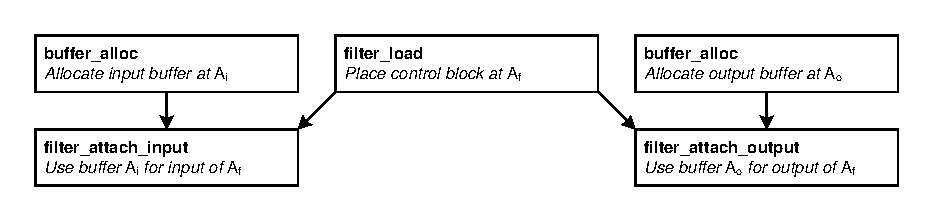
\includegraphics[scale=.55]{figs/init}
\end{center}
\caption[Commands to set up a filter.]{Commands to load a filter and allocate and attach input and output buffers. Lines between commands represent dependencies that must be specified to the library when the commands are issued. These commands may be issued in one or multiple groups.}
\label{fig:lib:init}
\end{figure}

In addition, input data must be transferred into the input buffer before the filter can be run, and output data must eventually be transferred out of the output buffer. With an initially empty input buffer, the commands to transfer in $n$ iterations of input, run the filter for $n$ iterations, and then transfer out $n$ iterations of output (assuming that the input and output buffers were sized appropriately) are shown in Figure~\ref{fig:lib:run}.

\begin{figure}[!htb]
\begin{center}
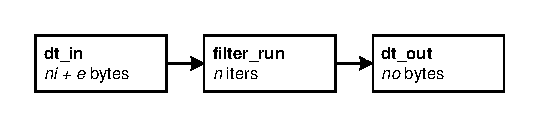
\includegraphics{figs/run}
\end{center}
\caption[Commands to run a filter.]{Commands to run a filter for the
  first $n$ iterations, including transferring input and output. The
  corresponding data transfer commands on other cores are not shown.}
\label{fig:lib:run}
\end{figure}

A sequence of commands is required to run the filter for a larger
number of iterations on a core with a finite local store
capacity. This is illustrated in Figure~\ref{fig:lib:ext}.

\begin{figure}[!htb]
\begin{center}
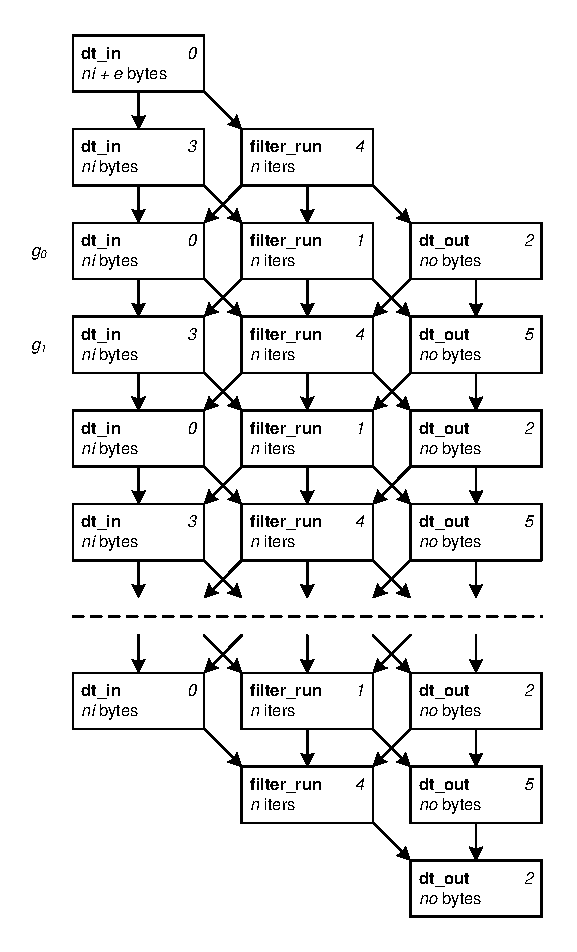
\includegraphics[scale=.90]{figs/ext}
\end{center}
\caption[Sequence of commands to run a filter for a large number of iterations.]{Sequence of commands to run a filter for a large number of iterations. Command IDs are indicated in the upper right. Each row is issued as a different group.}
\label{fig:lib:ext}
\end{figure}

Provided that the input buffer is at least $2ni+e$ bytes and the output buffer is at least $2no$ bytes, the dependencies among the commands in the sequence ensure that:
\begin{itemize}
\item When a \textsf{dt\_in} command becomes active, there are at most $ni+e$ bytes of data in the input buffer, and thus enough space to transfer in an additional $ni$ bytes.
\item When a \textsf{dt\_out} command becomes active, there are at least $no$ bytes of data in the output buffer, and thus enough data to transfer out.
\item When a \textsf{filter\_run} command becomes active, there are at least $ni+e$ bytes of data in the input buffer and at most $no$ bytes of data in the output buffer. This is enough input data and output space to run the filter for $n$ iterations.
\end{itemize}

This sequence of commands effectively ``pipelines'' the basic operation from Figure~\ref{fig:lib:run}. Double-buffering is accomplished when the data transfer commands in a group complete before the \textsf{filter\_run} does. In this case, the following \textsf{filter\_run} has no outstanding dependencies once the current \textsf{filter\_run} completes, and can become active immediately.

The user or scheduler can keep the core continually supplied with work
by initially issuing the first two groups, thereafter issuing the next
group whenever a group completes. In this case, the core almost always
has two groups of commands issued, with one group active and the other
queued. In addition, with the exception of the first two and last two
groups, the command parameters, IDs and dependencies in every other
group are identical. This allows the user to initially set up two
groups ($g_0$ and $g_1$ in Figure~\ref{fig:lib:ext}) and repeatedly
issue them for a majority of the execution. If executions are
relatively long, the overhead of the first and last group, where no
filter is being run, will be amortized effectively. Alternatively, the
user can load another filter and run it during those gaps.

In practice, situations such as the above, where a static-rate filter
is run for a large number of iterations and large amounts of input and
output data are transferred, are very common in streaming code. To
avoid requiring the user to manually issue groups and deal with
command completion callbacks in every such case, the MSL library also
provides extended operations that encapsulate this pattern. In an
extended operation, the user provides the library with filter rates,
the addresses of opposing buffers on other processors for data
transfers, and the number of groups to run for; the library issues and
responds to all commands internally and notifies the user when the
entire operation is complete.
%% Where one or both opposing buffers are located in memory,
%% the library also handles the PPE side of data transfers
%% internally. 
Extended operations greatly simplify setting up pipelines
of any length where all filters in the pipeline have static rates.


  \section{Conclusions and Future Work}
\label{sec:conclusion}

This paper makes two contributions.  First, it introduces teleport
messaging: a powerful language construct enabling precise message
delivery between nodes of a distributed stream program.  In comparison
with other methods to implement messaging functionality in a
Synchronous Dataflow (SDF) model, teleport messaging is arguably more
readable, more robust, and easier to maintain.  In addition, our
implementation of teleport messaging in the StreamIt compiler resulted
in a 49\% performance improvement for a frequency hopping radio
running on a cluster of workstations.  Like several declarative
language constructs, teleport messaging improves performance by
exposing the true dependences to the compiler and allowing it to
optimize the communication.

%% We outlined several possible applications of $\sdep$, including
%% latency constraints, debugging, speculation, and program analysis, and
%% we look forward to pursuing these directions in the future.

Second, this paper formulates $\sdep$, a natural and useful dependence
representation for the streaming domain.  While this paper applies
$\sdep$ to a new language construct, we envision other applications as
well.  For example, $\sdep$ could be used in a debugger to identify
which iterations of an upstream actor are affecting a given iteration
of a downstream actor.  In a software-based speculation
system~\cite{frank-thesis}, $\sdep$ could be applied to trace the
effects of a failed prediction and to roll back the appropriate actor
executions.  $\sdep$ also offers a new method for measuring latency in
a stream graph.  Similar to representations such as dependence
levels~~\cite{AK82}, direction vectors~\cite{wolfe82}, and dependence
polyhedra~\cite{Irig88} for scientific programs, $\sdep$ provides
dependence information that could be used to test or verify program
transformations.

There are some limitations in the current study that are fertile
grounds for future research.  First, our formulation of $\sdep$
requires a directed path in the stream graph (aligned with the
direction of data flow) between the actors in question.  We are
generalizing $\sdep$ to actors that run in parallel by leveraging
their data dependences with common predecessors (upstream) or
successors (downstream).  Second, as detailed in
Section~\ref{sec:constraints}, we do not solve the general scheduling
problem that incorporates overlapping constraints from teleport
messaging; even determining whether or not a set of constraints is
feasible (especially during the initialization
schedule~\cite{karczma-thesis}) seems to be an interesting question.
Third, in the current model only actors can send and receive messages.
We are extending this into a hierarchical model where stream
containers (such as pipelines) can also receive events and dispatch
them precisely to other streams.  Finally, our approach relies on the
static communication rates present in SDF.  It would be interesting to
consider teleport messaging in a more dynamic context; for example,
downstream non-negative latency messages could be immediately
supported by embedding messages in data items, while other messages
might require speculative delivery or modified timing contracts.

Our work can be viewed as the integration of dynamic behavior into a
static dataflow language.  Our insight is that there is a class of
control messages that only adjust a parameter in the target actor;
they do not otherwise affect the input or output channels upon
delivery.  This model enables a hybrid scheduling scheme in which the
steady-state dataflow is exactly orchestrated at compile time, but
there are windows in which a message could adjust an internal field of
an actor between its execution steps.  We consider this to be a
promising avenue for creating a unified development environment that
captures all aspects of stream application development without
sacrificing either performance or programmability.


  \bibliographystyle{abbrv}
  \bibliography{references}

  \section*{Appendix: Alpha Code}
\todo{Insert final example.a file in verbatim here}

  
\end{document}